\section {Setting the IP address}

In this section we deal with setting the IP address.

The site player has been given a default IP address of 10.100.100.100 so it initially
starts on 10.100.100.100. The IP address
can also be set by the PIC chip configuration to overide this value.

The IP address may also of been set to another value at factory and then locked down, to change it the unit
will need returning to factory.

\subsection{Setting the IP address using Web Interface}

To set the IP address you need to be logged into the WebBrick.  This is done by selecting the login page , 
from the menu and then entering the level 2 or 3 password into the login field.

Select the Configure server and enter the new IP address into the correct 4 boxes and then click Save.

See section on Configure Server in Web Interface section.

\index{IP Address,Unknown}
If you are not sure what IP address the device is using, run either the WebBrickMon application which is a windows
application that can be downloaded from http://community.webbricksystems.com or use the python wbMonitor program. 
Both of these should pick up UDP events
being sent by the webBrick and display them. The IP address is listed after the time stamp on the Windows application.

\subsection{Setting the IP address using Python}
There is a python fragment setIp.py that can be edited and used to set the IP address, it needs the MAC address and new 
IP address installing in it. It is only intended to be used where the WebBrick is on its default of 10.100.100.100, 
possibly with other new WebBricks. This is the basis of the home gateway Discovery activity.

\subsection{Setting the IP address using WebBrickMon}
WebBrickMon is a standalone windows application, it's primary purpose is for use in 
initial setup to locate your webbrick on your local network. It communicates with a webbrick to set the IP address
using broadcast messages and therefore can work when you caannot access the web interface.

When the monitor is started you will see something similar to this:

\begin{figure}[H]
\centering
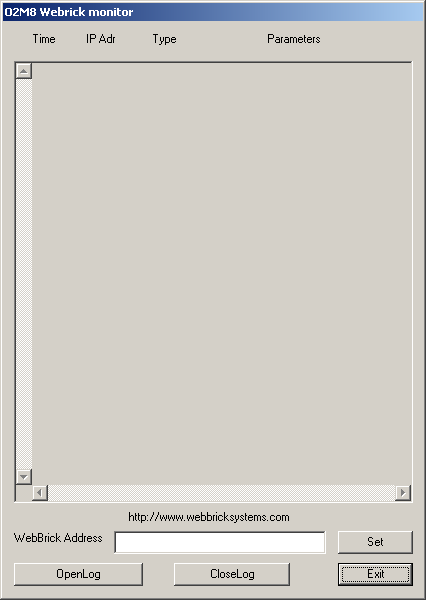
\includegraphics[width=0.8\textwidth]{Images/WebBrickMon.png}
\end{figure}

The top section shows UDP events coming from the webbrick, if your network is capable of connecting to the IP
address listed in the events then just use your web browser to connect to the IP address. If your system uses 
different IP address ranges then enter aa new IP address in the box at the bottom labelled WebBrickAddress and
click SET. The monitor will then wait for the next NewNode event and change its webbrick address. You should then
see the IP address in the events change.


\begin{figure}[H]
\centering
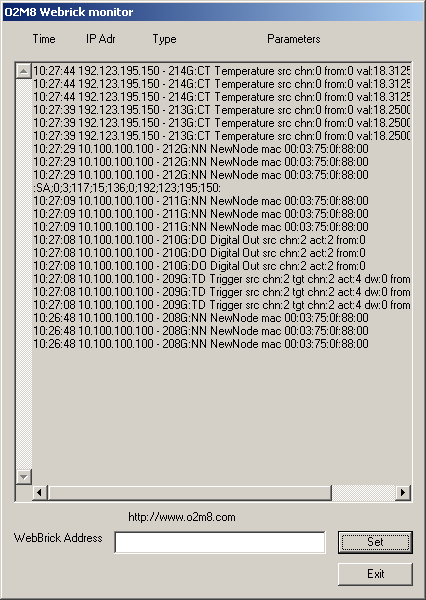
\includegraphics[width=0.8\textwidth]{Images/WebBrickMon2.png}
\end{figure}

